\documentclass[11pt,a4paper]{article}

% =========================================================================
% PACKAGES & ENGINE SETUP
% =========================================================================
\usepackage[utf8]{inputenc}
\usepackage[margin=1in]{geometry}
\usepackage{microtype}
\usepackage{amsmath,amssymb,mathtools,bm}
\usepackage{booktabs,tabularx,multirow}
\usepackage{xcolor}
\usepackage{hyperref}
\usepackage{listings}
\usepackage{tikz}
\usetikzlibrary{shapes.geometric,arrows.meta,positioning,calc,backgrounds,fit,decorations.pathreplacing}
\usepackage[most]{tcolorbox}

% =========================================================================
% COLOR PALETTE (Modern Editorial Academic)
% =========================================================================
\definecolor{primary}{RGB}{18, 52, 86}       % Deep Prussian Blue
\definecolor{secondary}{RGB}{30, 114, 133}   % Ocean Teal
\definecolor{accent}{RGB}{196, 69, 54}       % Crimson / Warning
\definecolor{bglight}{RGB}{248, 250, 252}    % Soft Canvas Slate
\definecolor{borderlight}{RGB}{226, 232, 240}
\definecolor{boxgreen}{RGB}{40, 167, 69}
\definecolor{boxpurple}{RGB}{111, 66, 193}
\definecolor{boxamber}{RGB}{217, 119, 6}

% Hyperref setup
\hypersetup{
    colorlinks=true,
    linkcolor=primary,
    citecolor=secondary,
    urlcolor=secondary,
    pdftitle={A Rigorous Introduction to Machine Learning, Deep Learning, and Large Language Models},
    pdfauthor={Systems & AI Research Lab}
}

% =========================================================================
% CUSTOM TCOLORBOX ENVIRONMENTS
% =========================================================================
\newtcolorbox{conceptbox}[1]{
    enhanced,
    colback=bglight,
    colframe=secondary,
    coltitle=white,
    fonttitle=\bfseries,
    title={#1},
    arc=4mm,
    boxrule=1pt,
    left=4mm, right=4mm, top=3mm, bottom=3mm,
    drop shadow=black!10
}

\newtcolorbox{mathbox}[1]{
    enhanced,
    colback=white,
    colframe=primary,
    coltitle=white,
    fonttitle=\bfseries\small,
    title={#1},
    arc=2mm,
    boxrule=0.8pt,
    left=3mm, right=3mm, top=2mm, bottom=2mm
}

\newtcolorbox{warningbox}[1]{
    enhanced,
    colback=accent!5!white,
    colframe=accent,
    coltitle=white,
    fonttitle=\bfseries,
    title={#1},
    arc=3mm,
    boxrule=1pt
}

% Code Listings Styling
\lstset{
    basicstyle=\ttfamily\small,
    backgroundcolor=\color{bglight},
    frame=single,
    rulecolor=\color{borderlight},
    keywordstyle=\color{primary}\bfseries,
    commentstyle=\color{gray}\itshape,
    stringstyle=\color{secondary},
    breaklines=true,
    numbers=none
}

% =========================================================================
% DOCUMENT METADATA
% =========================================================================
\title{
    \vspace{-1.5cm}
    \textbf{\huge From Perceptrons to Pre-Trained Transformers} \\[0.3cm]
    \large A Mathematical \& Systems Introduction to Machine Learning, Deep Learning, and LLMs
}
\author{\textbf{Autonomous Systems \& Neural Foundations Engineering}}
\date{\today}

\begin{document}
\maketitle

\begin{abstract}
This monograph provides an end-to-end, mathematically rigorous yet visually intuitive introduction to the hierarchy of modern artificial intelligence: Classical Machine Learning (ML), Deep Neural Representations (DL), and Large Language Models (LLMs). We dissect learning paradigms, optimization algorithms, gradient-based dynamics, statistical evaluation metrics (Confusion Matrix, Precision/Recall, $F_1$, Z-scores, K-Fold cross-validation), the Transformer self-attention mechanism, Grouped-Query Attention (GQA), and decentralized pre-training from zero weights. Complete with self-contained vector TikZ diagrams, this reference is designed for computer scientists, systems programmers, and machine learning practitioners.
\end{abstract}

\tableofcontents
\vspace{0.8cm}
\hrule
\vspace{0.8cm}

% =========================================================================
% SECTION 1: THE TAXONOMY OF LEARNING
% =========================================================================
\section{The AI Hierarchy: Foundations \& Taxonomy}

Artificial Intelligence is organized as concentric paradigms, where each domain builds directly on the mathematical primitives of its predecessor.

\begin{figure}[htbp]
\centering
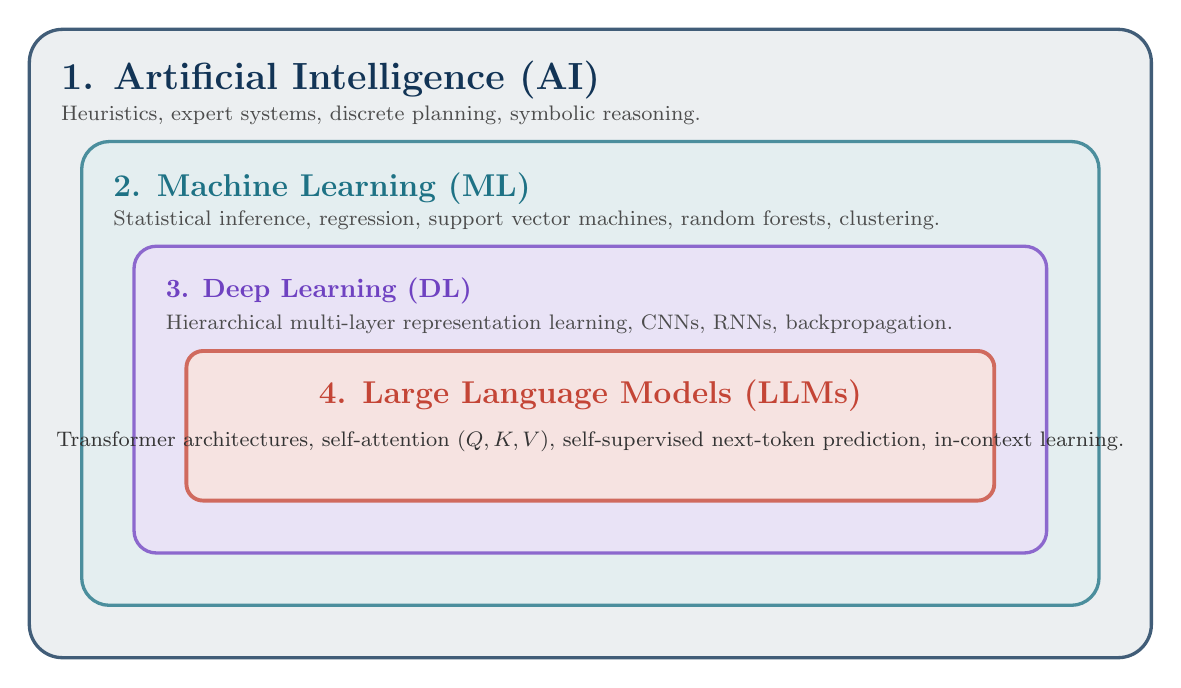
\begin{tikzpicture}[scale=0.95, every node/.style={transform shape}]
    % Outer Layer: Artificial Intelligence
    \draw[fill=primary!8, draw=primary!80, line width=1.2pt, rounded corners=12pt] 
        (-7.5, -4.2) rectangle (7.5, 4.2);
    \node[anchor=north west, font=\bfseries\color{primary}] at (-7.2, 3.9) 
        {\Large \textbf{1. Artificial Intelligence (AI)}};
    \node[anchor=north west, font=\footnotesize\color{black!70}] at (-7.2, 3.3) 
        {Heuristics, expert systems, discrete planning, symbolic reasoning.};

    % Layer 2: Machine Learning
    \draw[fill=secondary!12, draw=secondary!80, line width=1.2pt, rounded corners=10pt] 
        (-6.8, -3.5) rectangle (6.8, 2.7);
    \node[anchor=north west, font=\bfseries\color{secondary}] at (-6.5, 2.4) 
        {\large \textbf{2. Machine Learning (ML)}};
    \node[anchor=north west, font=\footnotesize\color{black!70}] at (-6.5, 1.9) 
        {Statistical inference, regression, support vector machines, random forests, clustering.};

    % Layer 3: Deep Learning
    \draw[fill=boxpurple!15, draw=boxpurple!80, line width=1.2pt, rounded corners=8pt] 
        (-6.1, -2.8) rectangle (6.1, 1.3);
    \node[anchor=north west, font=\bfseries\color{boxpurple}] at (-5.8, 1.0) 
        {\textbf{3. Deep Learning (DL)}};
    \node[anchor=north west, font=\footnotesize\color{black!70}] at (-5.8, 0.5) 
        {Hierarchical multi-layer representation learning, CNNs, RNNs, backpropagation.};

    % Layer 4: Large Language Models
    \draw[fill=accent!15, draw=accent!80, line width=1.4pt, rounded corners=6pt] 
        (-5.4, -2.1) rectangle (5.4, -0.1);
    \node[anchor=center, font=\bfseries\large\color{accent}] at (0, -0.7) 
        {\textbf{4. Large Language Models (LLMs)}};
    \node[anchor=center, font=\footnotesize\color{black!80}] at (0, -1.3) 
        {Transformer architectures, self-attention ($Q, K, V$), self-supervised next-token prediction, in-context learning.};
\end{tikzpicture}
\caption{The Architectural Hierarchy: From Symbolic AI to Foundation LLMs.}
\label{fig:ai_hierarchy}
\end{figure}

\subsection{Core Learning Paradigms}
Machine learning algorithms are classified into three primary operational paradigms:

\begin{enumerate}
    \item \textbf{Supervised Learning}: Given a dataset $\mathcal{D} = \{(\bm{x}_i, y_i)\}_{i=1}^N$ of features $\bm{x}_i \in \mathbb{R}^d$ and ground-truth targets $y_i$, find a parameterized mapping $f_{\bm{\theta}}: \mathbb{R}^d \to \mathcal{Y}$ that minimizes empirical risk:
    \begin{equation}
        \mathcal{R}_{\text{emp}}(\bm{\theta}) = \frac{1}{N} \sum_{i=1}^N \mathcal{L}(f_{\bm{\theta}}(\bm{x}_i), y_i)
    \end{equation}
    \item \textbf{Unsupervised Learning}: Given unlabeled observations $\mathcal{D} = \{\bm{x}_i\}_{i=1}^N$, infer latent structures, cluster assignments, or low-dimensional manifolds without ground-truth labels ($p(\bm{x})$).
    \item \textbf{Self-Supervised Learning (Foundation of LLMs)}: Targets are generated automatically from the structure of the data itself. For language modeling, given a token stream $(w_1, w_2, \dots, w_T)$, the task is autoregressive next-token prediction:
    \begin{equation}
        \max_{\bm{\theta}} \sum_{t=1}^T \log P(w_t \mid w_1, w_2, \dots, w_{t-1}; \bm{\theta})
    \end{equation}
\end{enumerate}

% =========================================================================
% SECTION 2: TRAINING DYNAMICS: EPOCH, BATCH, ITERATION
% =========================================================================
\section{Training Dynamics: Epochs, Batches, and Iterations}

A common source of confusion in optimization is the relationship between an \textit{Epoch}, a \textit{Batch}, and an \textit{Iteration (Step)}.

\begin{conceptbox}{Definitions at a Glance}
\begin{itemize}
    \item \textbf{Batch Size ($B$)}: The number of distinct input sequences processed in parallel across compute cores before performing a gradient update.
    \item \textbf{Iteration / Step ($S$)}: Exactly \textbf{one parameter update} via gradient backpropagation:
    $$\bm{\theta}_{t+1} \leftarrow \bm{\theta}_t - \eta \cdot \nabla_{\bm{\theta}} \mathcal{L}_B(\bm{\theta}_t)$$
    \item \textbf{Epoch ($E$)}: Exactly \textbf{one complete traversal} over every sample in the training corpus:
    $$\text{Iterations per Epoch} = \left\lceil \frac{N_{\text{total}}}{B_{\text{effective}}} \right\rceil$$
\end{itemize}
\end{conceptbox}

\begin{figure}[htbp]
\centering
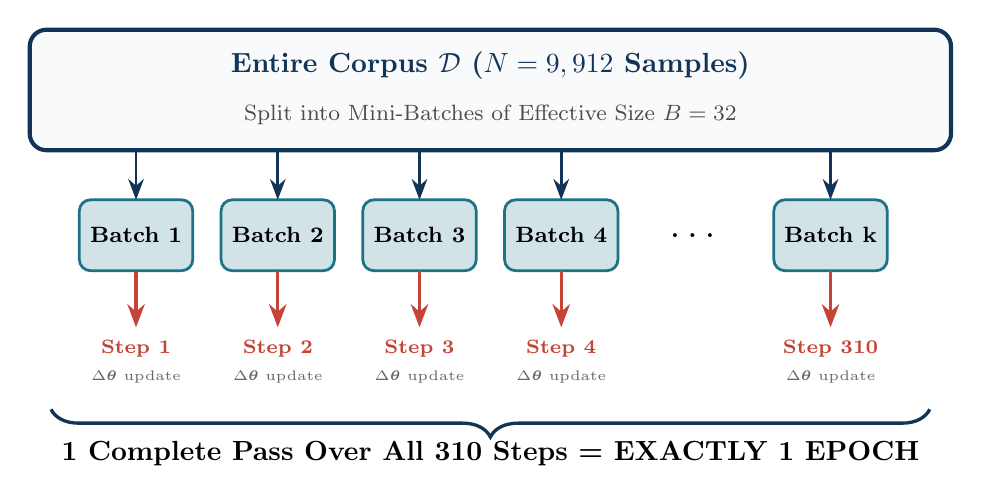
\begin{tikzpicture}[scale=0.9]
    % Entire Dataset Box
    \draw[fill=bglight, draw=primary, line width=1.5pt, rounded corners=6pt] (-6.5, 2.5) rectangle (6.5, 4.2);
    \node[font=\bfseries\color{primary}] at (0, 3.7) {Entire Corpus $\mathcal{D}$ ($N = 9,912$ Samples)};
    \node[font=\footnotesize\color{black!70}] at (0, 3.0) {Split into Mini-Batches of Effective Size $B = 32$};

    % Batches
    \foreach \i/\x in {1/-5, 2/-3, 3/-1, 4/1, k/4.8} {
        \draw[fill=secondary!20, draw=secondary, line width=1pt, rounded corners=4pt] (\x-0.8, 0.8) rectangle (\x+0.8, 1.8);
        \ifx\i\string k
            \node[font=\footnotesize\bfseries] at (\x, 1.3) {Batch 310};
        \else
            \node[font=\footnotesize\bfseries] at (\x, 1.3) {Batch \i};
        \fi
        \draw[-Stealth, primary, line width=1pt] (\x, 2.5) -- (\x, 1.8);
    }
    \node[font=\Large\bfseries] at (2.9, 1.3) {$\dots$};

    % Arrows to Steps
    \foreach \x/\step in {-5/Step 1, -3/Step 2, -1/Step 3, 1/Step 4, 4.8/Step 310} {
        \draw[-Stealth, accent, line width=1.2pt] (\x, 0.8) -- (\x, 0.0);
        \node[font=\scriptsize\bfseries\color{accent}] at (\x, -0.3) {\step};
        \node[font=\tiny\color{black!60}] at (\x, -0.7) {$\Delta \bm{\theta}$ update};
    }

    % Full Epoch Bracket
    \draw [decorate, decoration={brace, amplitude=10pt, mirror, raise=4pt}, line width=1.2pt, color=primary]
        (-6.2, -1.0) -- (6.2, -1.0) node [black, midway, yshift=-0.7cm, font=\bfseries] 
        {1 Complete Pass Over All 310 Steps = EXACTLY 1 EPOCH};
\end{tikzpicture}
\caption{The Decomposition of an Epoch into Discrete Optimization Iterations.}
\label{fig:epoch_diagram}
\end{figure}

% =========================================================================
% SECTION 3: EVALUATION METRICS & DIAGNOSTIC STATISTICS
% =========================================================================
\section{Diagnostic Metrics, Statistical Scores \& Validation}

In systems diagnostics, intrusion detection, and classification, raw accuracy is frequently misleading due to severe class imbalance.

\subsection{The Visual Confusion Matrix}
Every binary decision boundary induces four distinct event classes. Figure~\ref{fig:confusion_matrix} maps how Precision, Recall, and Accuracy are partitioned from this matrix.

\begin{figure}[htbp]
\centering
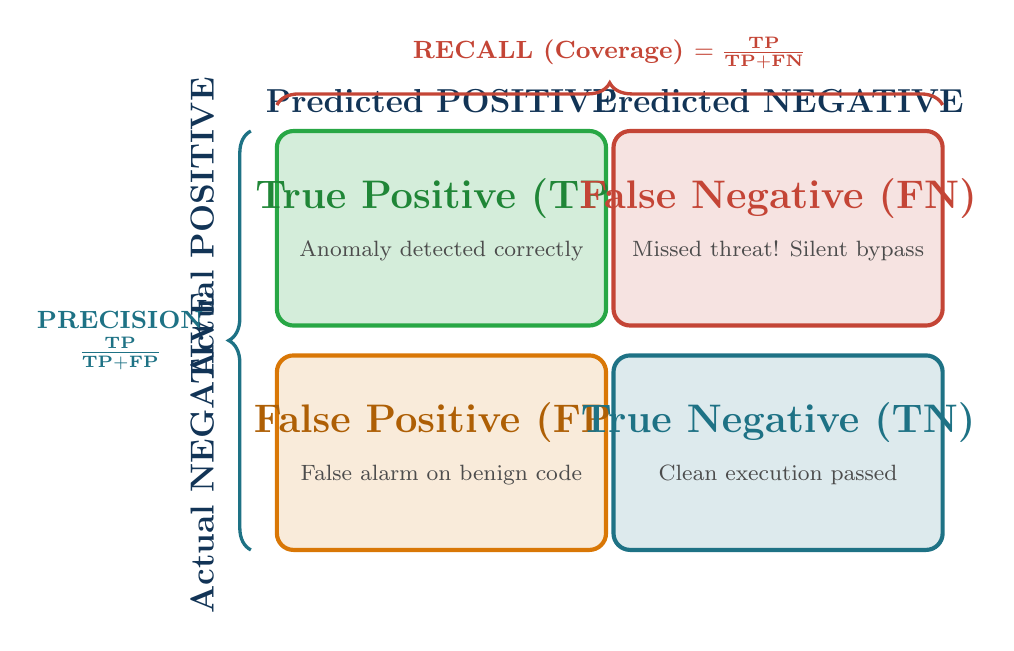
\begin{tikzpicture}[scale=0.95]
    % Header labels
    \node[font=\bfseries\large\color{primary}] at (0, 3.2) {Predicted POSITIVE};
    \node[font=\bfseries\large\color{primary}] at (4.5, 3.2) {Predicted NEGATIVE};
    
    \node[font=\bfseries\large\color{primary}, rotate=90] at (-3.2, 1.5) {Actual POSITIVE};
    \node[font=\bfseries\large\color{primary}, rotate=90] at (-3.2, -1.5) {Actual NEGATIVE};

    % TP Box
    \draw[fill=boxgreen!20, draw=boxgreen, line width=1.5pt, rounded corners=6pt] (-2.2, 0.2) rectangle (2.2, 2.8);
    \node[font=\Large\bfseries\color{boxgreen!80!black}] at (0, 1.9) {True Positive (TP)};
    \node[font=\footnotesize\color{black!70}] at (0, 1.2) {Anomaly detected correctly};

    % FN Box
    \draw[fill=accent!15, draw=accent, line width=1.5pt, rounded corners=6pt] (2.3, 0.2) rectangle (6.7, 2.8);
    \node[font=\Large\bfseries\color{accent}] at (4.5, 1.9) {False Negative (FN)};
    \node[font=\footnotesize\color{black!70}] at (4.5, 1.2) {Missed threat! Silent bypass};

    % FP Box
    \draw[fill=boxamber!15, draw=boxamber, line width=1.5pt, rounded corners=6pt] (-2.2, -2.8) rectangle (2.2, -0.2);
    \node[font=\Large\bfseries\color{boxamber!80!black}] at (0, -1.1) {False Positive (FP)};
    \node[font=\footnotesize\color{black!70}] at (0, -1.8) {False alarm on benign code};

    % TN Box
    \draw[fill=secondary!15, draw=secondary, line width=1.5pt, rounded corners=6pt] (2.3, -2.8) rectangle (6.7, -0.2);
    \node[font=\Large\bfseries\color{secondary}] at (4.5, -1.1) {True Negative (TN)};
    \node[font=\footnotesize\color{black!70}] at (4.5, -1.8) {Clean execution passed};

    % Precision Bracket (Vertical slice of column 1)
    \draw [decorate, decoration={brace, amplitude=8pt, mirror, raise=4pt}, line width=1.2pt, color=secondary]
        (-2.4, 2.8) -- (-2.4, -2.8) node [secondary, midway, xshift=-1.8cm, font=\bfseries\small, align=center] 
        {\textbf{PRECISION}\\$\frac{\text{TP}}{\text{TP} + \text{FP}}$};

    % Recall Bracket (Horizontal slice of row 1)
    \draw [decorate, decoration={brace, amplitude=8pt, raise=4pt}, line width=1.2pt, color=accent]
        (-2.2, 3.0) -- (6.7, 3.0) node [accent, midway, yshift=0.8cm, font=\bfseries\small, align=center] 
        {\textbf{RECALL (Coverage)} $= \frac{\text{TP}}{\text{TP} + \text{FN}}$};
\end{tikzpicture}
\caption{The Geometry of Precision and Recall on the Confusion Matrix.}
\label{fig:confusion_matrix}
\end{figure}

\subsection{Precision, Recall, and the $F_1$ Score}

\begin{mathbox}{Fundamental Classification Formulas}
\begin{align}
    \text{Accuracy} &= \frac{\text{TP} + \text{TN}}{\text{TP} + \text{TN} + \text{FP} + \text{FN}} \\[0.2cm]
    \text{Precision (Positive Predictive Value)} &= \frac{\text{TP}}{\text{TP} + \text{FP}} \quad \text{(\textit{Alert Reliability})} \\[0.2cm]
    \text{Recall (Sensitivity / True Positive Rate)} &= \frac{\text{TP}}{\text{TP} + \text{FN}} \quad \text{(\textit{Threat Coverage})} \\[0.2cm]
    F_1 \text{ Score (Harmonic Mean)} &= 2 \cdot \frac{\text{Precision} \cdot \text{Recall}}{\text{Precision} + \text{Recall}} = \frac{2\text{TP}}{2\text{TP} + \text{FP} + \text{FN}}
\end{align}
\end{mathbox}

\noindent \textbf{Why the Harmonic Mean?} The arithmetic mean of $P=1.0$ and $R=0.0$ yields $0.5$, masquerading as moderate performance. The harmonic mean forces $F_1 \to 0$ whenever either metric collapses:
\begin{equation}
    F_\beta = (1 + \beta^2) \frac{\text{Precision} \cdot \text{Recall}}{(\beta^2 \cdot \text{Precision}) + \text{Recall}}
\end{equation}
When missing an event is catastrophic (e.g., zero-day exploit detection), we select $\beta = 2$ ($F_2$ score) to weight Recall twice as heavily as Precision.

\subsection{K-Fold Cross-Validation}
To avoid evaluation bias on arbitrary train-test splits, the dataset $\mathcal{D}$ is partitioned into $K$ disjoint subsets $\mathcal{D}_1, \dots, \mathcal{D}_K$. Figure~\ref{fig:kfold} illustrates how every partition serves as an unseen test benchmark.

\begin{figure}[htbp]
\centering
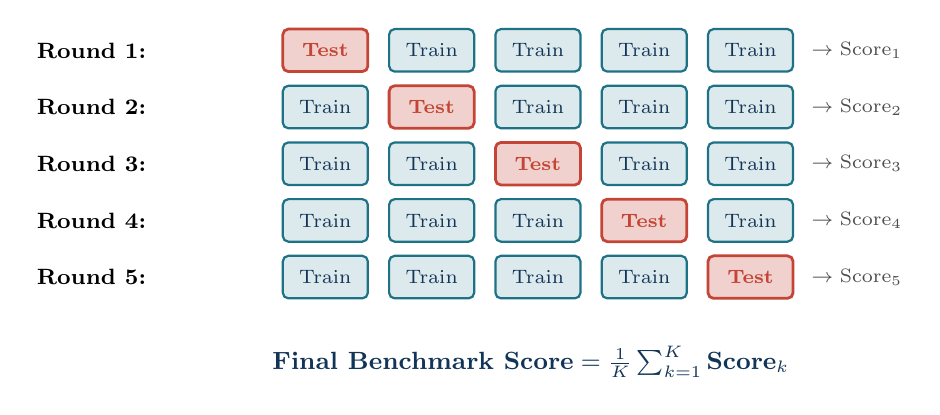
\begin{tikzpicture}[scale=0.9]
    \foreach \fold/\val in {1/1, 2/2, 3/3, 4/4, 5/5} {
        \node[font=\footnotesize\bfseries] at (-1.2, {-\fold*0.8}) {Round \fold:};
        \foreach \block in {1, 2, 3, 4, 5} {
            \ifnum\block=\val
                \draw[fill=accent!25, draw=accent, line width=1pt, rounded corners=2pt] 
                    ({\block*1.5}, {-\fold*0.8-0.3}) rectangle ({\block*1.5+1.2}, {-\fold*0.8+0.3});
                \node[font=\scriptsize\bfseries\color{accent}] at ({\block*1.5+0.6}, {-\fold*0.8}) {Test};
            \else
                \draw[fill=secondary!15, draw=secondary, line width=0.8pt, rounded corners=2pt] 
                    ({\block*1.5}, {-\fold*0.8-0.3}) rectangle ({\block*1.5+1.2}, {-\fold*0.8+0.3});
                \node[font=\scriptsize\color{primary}] at ({\block*1.5+0.6}, {-\fold*0.8}) {Train};
            \fi
        }
        \node[font=\scriptsize\color{black!70}] at (9.6, {-\fold*0.8}) {$\to \text{Score}_{\fold}$};
    }
    \node[font=\small\bfseries\color{primary}] at (5.0, -5.2) 
        {$\text{Final Benchmark Score} = \frac{1}{K}\sum_{k=1}^K \text{Score}_k$};
\end{tikzpicture}
\caption{K-Fold Cross-Validation: Every sample is evaluated in held-out test data.}
\label{fig:kfold}
\end{figure}

\subsection{Standardization via Z-Scores}
In anomaly detection, a Z-score measures how many standard deviations an observation $x$ deviates from the baseline mean $\mu$:
\begin{equation}
    z = \frac{x - \mu}{\sigma}
\end{equation}

\begin{figure}[htbp]
\centering
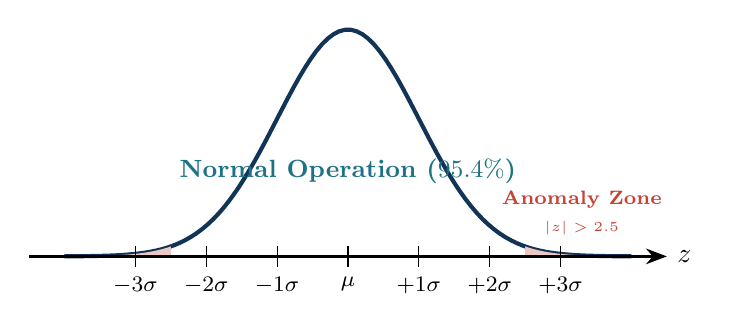
\begin{tikzpicture}[scale=0.9]
    % Gaussian curve
    \draw[line width=1.5pt, primary, domain=-4:4, samples=100] 
        plot (\x, {3.2*exp(-\x*\x/2)});

    % Fill anomaly tails
    \fill[accent!30, domain=2.5:4] 
        plot (\x, {3.2*exp(-\x*\x/2)}) -- (4,0) -- (2.5,0) -- cycle;
    \fill[accent!30, domain=-4:-2.5] 
        (-4,0) -- plot (\x, {3.2*exp(-\x*\x/2)}) -- (-2.5,0) -- cycle;

    % Axis
    \draw[-Stealth, line width=1pt] (-4.5, 0) -- (4.5, 0) node[right] {$z$};
    
    % Ticks
    \foreach \z/\label in {-3/-3\sigma, -2/-2\sigma, -1/-1\sigma, 0/\mu, 1/+1\sigma, 2/+2\sigma, 3/+3\sigma} {
        \draw (\z, 0.15) -- (\z, -0.15);
        \node[font=\footnotesize, below=4pt] at (\z, 0) {$\label$};
    }

    % Normal regions
    \node[font=\bfseries\small\color{secondary}] at (0, 1.2) {Normal Operation ($95.4\%$)};
    \node[font=\scriptsize\bfseries\color{accent}] at (3.3, 0.8) {Anomaly Zone};
    \node[font=\tiny\color{accent}] at (3.3, 0.4) {$|z| > 2.5$};
\end{tikzpicture}
\caption{The Standard Normal Distribution and Statistical Z-Score Thresholds.}
\label{fig:z_score}
\end{figure}

Under a normal distribution $\mathcal{N}(\mu, \sigma^2)$, values where $|z| > 3.0$ represent extreme tail events ($p < 0.0027$), flagging unauthorized runtime hooks, anomalous latency spikes, or structural shifts.

% =========================================================================
% SECTION 4: DEEP LEARNING & THE TRANSFORMER ARCHITECTURE
% =========================================================================
\section{Deep Representations: The Transformer Engine}

Modern foundation models abandon recurrence (RNN/LSTM) in favor of the fully parallelizable \textbf{Self-Attention} mechanism.

\begin{figure}[htbp]
\centering
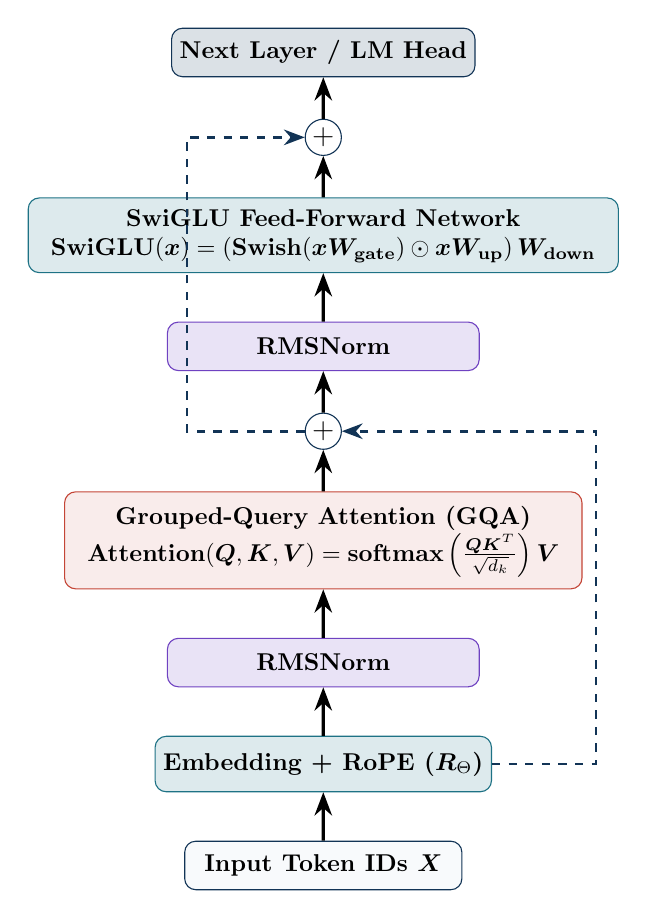
\begin{tikzpicture}[scale=0.88, every node/.style={transform shape}]
    % Input Embedding
    \node[draw=primary, fill=bglight, rounded corners, minimum width=4cm, minimum height=0.7cm, font=\bfseries] (inp) at (0, 0) {Input Token IDs $\bm{X}$};

    % Token + RoPE
    \node[draw=secondary, fill=secondary!15, rounded corners, minimum width=4.5cm, minimum height=0.8cm, font=\bfseries, above=0.7cm of inp] (emb) {Embedding + RoPE ($\bm{R}_\Theta$)};
    \draw[-Stealth, line width=1.2pt] (inp) -- (emb);

    % RMSNorm 1
    \node[draw=boxpurple, fill=boxpurple!15, rounded corners, minimum width=4.5cm, minimum height=0.7cm, font=\bfseries, above=0.7cm of emb] (norm1) {RMSNorm};
    \draw[-Stealth, line width=1.2pt] (emb) -- (norm1);

    % Attention Q K V
    \node[draw=accent, fill=accent!10, rounded corners, minimum width=5cm, minimum height=1.4cm, font=\bfseries, above=0.7cm of norm1] (attn) {
        \begin{tabular}{c}
            \textbf{Grouped-Query Attention (GQA)} \\
            $\text{Attention}(\bm{Q}, \bm{K}, \bm{V}) = \text{softmax}\left(\frac{\bm{Q}\bm{K}^T}{\sqrt{d_k}}\right)\bm{V}$
        \end{tabular}
    };
    \draw[-Stealth, line width=1.2pt] (norm1) -- (attn);

    % Residual Add 1
    \node[draw=primary, circle, fill=white, inner sep=1pt, font=\large\bfseries, above=0.6cm of attn] (add1) {$+$};
    \draw[-Stealth, line width=1.2pt] (attn) -- (add1);

    % Residual Skip Path 1
    \draw[-Stealth, line width=1pt, dashed, primary] (emb.east) -- ++(1.5,0) |- (add1.east);

    % RMSNorm 2
    \node[draw=boxpurple, fill=boxpurple!15, rounded corners, minimum width=4.5cm, minimum height=0.7cm, font=\bfseries, above=0.6cm of add1] (norm2) {RMSNorm};
    \draw[-Stealth, line width=1.2pt] (add1) -- (norm2);

    % SwiGLU MLP
    \node[draw=secondary, fill=secondary!15, rounded corners, minimum width=5cm, minimum height=1.0cm, font=\bfseries, above=0.7cm of norm2] (mlp) {
        \begin{tabular}{c}
            \textbf{SwiGLU Feed-Forward Network} \\
            $\text{SwiGLU}(\bm{x}) = \left(\text{Swish}(\bm{x}\bm{W}_{\text{gate}}) \odot \bm{x}\bm{W}_{\text{up}}\right)\bm{W}_{\text{down}}$
        \end{tabular}
    };
    \draw[-Stealth, line width=1.2pt] (norm2) -- (mlp);

    % Residual Add 2
    \node[draw=primary, circle, fill=white, inner sep=1pt, font=\large\bfseries, above=0.6cm of mlp] (add2) {$+$};
    \draw[-Stealth, line width=1.2pt] (mlp) -- (add2);

    % Residual Skip Path 2
    \draw[-Stealth, line width=1pt, dashed, primary] (add1.west) -- ++(-1.7,0) |- (add2.west);

    % Output
    \node[draw=primary, fill=primary!15, rounded corners, minimum width=4cm, minimum height=0.7cm, font=\bfseries, above=0.6cm of add2] (out) {Next Layer / LM Head};
    \draw[-Stealth, line width=1.2pt] (add2) -- (out);
\end{tikzpicture}
\caption{The Modern Pre-LayerNorm Transformer Block (LLaMA / DEMON Architecture).}
\label{fig:transformer_block}
\end{figure}

\subsection{Attention Evolution: MHA vs. MQA vs. GQA}
Standard Multi-Head Attention (MHA) maintains an independent Key and Value head for every Query head, causing massive Key-Value (KV) cache memory bloat during inference. Grouped-Query Attention (GQA) groups query heads to share a smaller number of KV heads:

\begin{figure}[htbp]
\centering
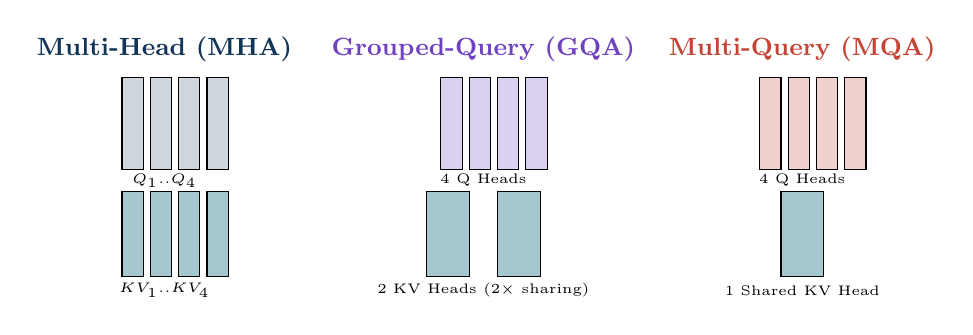
\begin{tikzpicture}[scale=0.9]
    % MHA
    \node[font=\bfseries\small\color{primary}] at (-4.5, 2.2) {Multi-Head (MHA)};
    \foreach \i in {1,2,3,4} {
        \draw[fill=primary!20] ({-5.5 + \i*0.4}, 0.5) rectangle ({-5.2 + \i*0.4}, 1.8);
        \draw[fill=secondary!40] ({-5.5 + \i*0.4}, -1.0) rectangle ({-5.2 + \i*0.4}, 0.2);
    }
    \node[font=\tiny] at (-4.5, 0.35) {$Q_1..Q_4$};
    \node[font=\tiny] at (-4.5, -1.2) {$KV_1..KV_4$};

    % GQA (Our setup)
    \node[font=\bfseries\small\color{boxpurple}] at (0, 2.2) {Grouped-Query (GQA)};
    \foreach \i in {1,2,3,4} {
        \draw[fill=boxpurple!25] ({-1.0 + \i*0.4}, 0.5) rectangle ({-0.7 + \i*0.4}, 1.8);
    }
    \draw[fill=secondary!40] (-0.8, -1.0) rectangle (-0.2, 0.2);
    \draw[fill=secondary!40] (0.2, -1.0) rectangle (0.8, 0.2);
    \node[font=\tiny] at (0, 0.35) {4 Q Heads};
    \node[font=\tiny] at (0, -1.2) {2 KV Heads ($2\times$ sharing)};

    % MQA
    \node[font=\bfseries\small\color{accent}] at (4.5, 2.2) {Multi-Query (MQA)};
    \foreach \i in {1,2,3,4} {
        \draw[fill=accent!25] ({3.5 + \i*0.4}, 0.5) rectangle ({3.8 + \i*0.4}, 1.8);
    }
    \draw[fill=secondary!40] (4.2, -1.0) rectangle (4.8, 0.2);
    \node[font=\tiny] at (4.5, 0.35) {4 Q Heads};
    \node[font=\tiny] at (4.5, -1.2) {1 Shared KV Head};
\end{tikzpicture}
\caption{Comparison of Attention KV Cache Footprints (GQA balances speed and memory).}
\label{fig:gqa_comparison}
\end{figure}

% =========================================================================
% SECTION 5: THE LLM LIFECYCLE
% =========================================================================
\section{The Complete Foundation Model Lifecycle}

\begin{figure}[htbp]
\centering
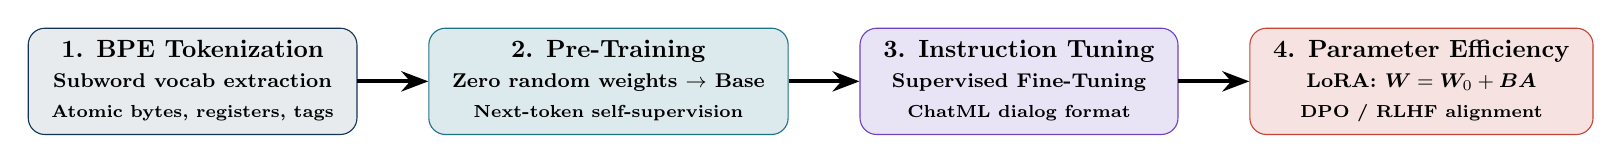
\begin{tikzpicture}[scale=0.9, node distance=1.6cm, every node/.style={transform shape}]
    % Step 1: Tokenizer
    \node[draw=primary, fill=primary!10, rounded corners=6pt, minimum width=3.5cm, minimum height=1.2cm, font=\bfseries] (tok) {
        \begin{tabular}{c}
            \textbf{1. BPE Tokenization} \\
            \footnotesize Subword vocab extraction \\
            \scriptsize Atomic bytes, registers, tags
        \end{tabular}
    };

    % Step 2: Pre-training
    \node[draw=secondary, fill=secondary!15, rounded corners=6pt, minimum width=3.5cm, minimum height=1.2cm, font=\bfseries, right=1.0cm of tok] (pre) {
        \begin{tabular}{c}
            \textbf{2. Pre-Training} \\
            \footnotesize Zero random weights $\to$ Base \\
            \scriptsize Next-token self-supervision
        \end{tabular}
    };
    \draw[-Stealth, line width=1.5pt] (tok) -- (pre);

    % Step 3: SFT
    \node[draw=boxpurple, fill=boxpurple!15, rounded corners=6pt, minimum width=3.5cm, minimum height=1.2cm, font=\bfseries, right=1.0cm of pre] (sft) {
        \begin{tabular}{c}
            \textbf{3. Instruction Tuning} \\
            \footnotesize Supervised Fine-Tuning \\
            \scriptsize ChatML dialog format
        \end{tabular}
    };
    \draw[-Stealth, line width=1.5pt] (pre) -- (sft);

    % Step 4: LoRA / Alignment
    \node[draw=accent, fill=accent!15, rounded corners=6pt, minimum width=3.5cm, minimum height=1.2cm, font=\bfseries, right=1.0cm of sft] (lora) {
        \begin{tabular}{c}
            \textbf{4. Parameter Efficiency} \\
            \footnotesize LoRA: $\bm{W} = \bm{W}_0 + \bm{B}\bm{A}$ \\
            \scriptsize DPO / RLHF alignment
        \end{tabular}
    };
    \draw[-Stealth, line width=1.5pt] (sft) -- (lora);
\end{tikzpicture}
\caption{The End-to-End Foundation Model Lifecycle.}
\label{fig:lifecycle}
\end{figure}

\subsection{Inference Decoding Strategies}
During autoregressive generation, logits $\bm{z}_t$ are converted to token probabilities via temperature scaling $T > 0$:
\begin{equation}
    P(w_i) = \frac{\exp(z_i / T)}{\sum_j \exp(z_j / T)}
\end{equation}
\begin{itemize}
    \item \textbf{Greedy ($T \to 0$)}: Always selects $\operatorname{argmax}_i z_i$. Completely deterministic.
    \item \textbf{Top-$k$ Sampling}: Truncates candidate pool to the $k$ most probable tokens.
    \item \textbf{Top-$p$ (Nucleus) Sampling}: Dynamically selects the smallest subset of tokens whose cumulative probability mass exceeds threshold $p$:
    \begin{equation}
        \sum_{i \in V^{(p)}} P(w_i) \ge p
    \end{equation}
\end{itemize}

% =========================================================================
% SECTION 6: SUMMARY FORMULARY
% =========================================================================
\section{Comprehensive Diagnostic Formulary}

\begin{table}[htbp]
\centering
\small
\renewcommand{\arraystretch}{1.4}
\begin{tabularx}{\textwidth}{l p{4.5cm} X}
\toprule
\textbf{Concept} & \textbf{Mathematical Formulation} & \textbf{Systems / Diagnostic Interpretation} \\
\midrule
\textbf{Precision} & $\frac{\text{TP}}{\text{TP} + \text{FP}}$ & Probability that an alert corresponds to an authentic anomaly. \\
\textbf{Recall} & $\frac{\text{TP}}{\text{TP} + \text{FN}}$ & Probability that a true anomaly is successfully intercepted. \\
\textbf{$F_1$ Score} & $\frac{2\text{TP}}{2\text{TP} + \text{FP} + \text{FN}}$ & Harmonic balance preventing over-optimization of false alarms or misses. \\
\textbf{Z-Score} & $z = \frac{x - \mu}{\sigma}$ & Distance from execution latency mean in units of standard deviation. \\
\textbf{Attention} & $\text{softmax}\left(\frac{\bm{Q}\bm{K}^T}{\sqrt{d_k}}\right)\bm{V}$ & Content-addressable soft associative memory across context tokens. \\
\textbf{SwiGLU} & $(\text{Swish}(\bm{x}\bm{W}_g) \odot \bm{x}\bm{W}_u)\bm{W}_d$ & Bilinear gating mechanism amplifying salient token representations. \\
\textbf{LoRA} & $\bm{W} = \bm{W}_0 + \frac{\alpha}{r}\bm{B}\bm{A}$ & Rank-$r$ decomposition reducing trainable parameter footprint by $>99\%$. \\
\bottomrule
\end{tabularx}
\caption{Core Formulations in Machine Learning and Language Architectures.}
\end{table}

\end{document}
